\subsection{Prioritize Requirements}\label{subsec:prioritize-requirements}

Another defining features of HelixRM is its ability to streamline and enhance the prioritization of requirements.
This functionality is designed to evaluate and rank requirements based on criteria such as business value, complexity, urgency, and risk.
By employing weighted scoring and customizable parameters, HelixRM ensures that stakeholders can make informed decisions that align with organizational goals and project constraints.

\paragraph{Establish Clear Evaluation Criteria}
HelixRM allows users to define and customize evaluation criteria to suit the unique needs of their projects.

\paragraph{Weighted Scoring}
The platform supports weighted scoring, enabling users to assign relative importance to each evaluation criterion.
This feature ensures that requirements are prioritized based on their significance to the project.

\paragraph{Automated Ranking}
HelixRM automates the ranking process, generating a prioritized list of requirements based on the established evaluation criteria and weighted scores.
This functionality saves time and minimizes subjectivity in the prioritization process.

\paragraph{Collaborative Decision-Making}
The platform facilitates collaborative decision-making by providing a transparent view of the prioritized requirements.
Stakeholders can review, discuss, and reach a consensus on the order of implementation.

\paragraph{Scenario Analysis}
HelixRM supports scenario analysis, allowing users to evaluate the impact of different prioritization strategies on project outcomes.
This feature enables stakeholders to make data-driven decisions that maximize project value.

\paragraph{Continuous Refinement}
As project requirements evolve, HelixRM enables users to continuously refine and update the prioritization of requirements.
This iterative process ensures that project goals remain aligned with changing business needs.
The image Figure~\ref{fig:requirements_view} shows an example of a prioritization of a requirement.
\begin{figure}[htpb]
    \centering
    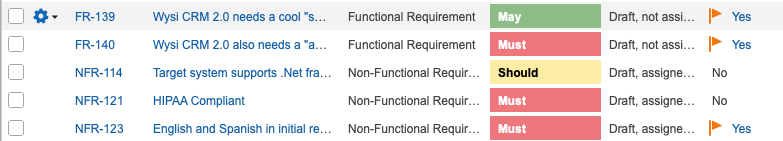
\includegraphics[width=\linewidth]{images/prioritize-example}
    \caption{Helix requirements view.}
    \label{fig:requirements_view}
\end{figure}